\chapter{Еще одно исследование наблюдаемости}
\label{ch:chap4}

\section{Условие задачи}

Рассматриваем систему:
$$
  \begin{cases}
    \dot{x} = Ax \\
    y = Cx
  \end{cases}
$$ и выполнить следующие шаги:
    
    \begin{itemize}
    \item Исследовать наблюдаемость системы, как в третьем задании
    \item  Определить, мог ли выход вида $y(t) = f(t)$ быть порожден начальными условиями, 
    отличными от найденных. Если да, то привести хотя бы три таких вектора
    начальных условий и выполнить для каждого из них (включая изначально най
    денный) моделирование, демонстрирующее корректность выполненных расчетов
    (одинаковые выходы при разном поведении векторов состояния систем).
    
    
    \end{itemize}


\section{Решение задачи}

Параметры для объекта:
$$
  A = \begin{bmatrix}
    8   &	-3	&  -12 \\
    -3   &   -2  &  -6 \\
    6  &    0  &  7
  \end{bmatrix} \tab
  C = \begin{bmatrix}
    0\\1\\1
  \end{bmatrix}^T \tab
  f(t) = 2e^{-2t}cos(3t) + e^{-2t}sin(3t)
$$



\subsection{Исследование наблюдаемости системы}
Для начала найдём матрицу наблюдаемости системы:
$$
V = \begin{bmatrix}
    C \\ CA \\ CA^2
\end{bmatrix} = \begin{bmatrix}
                0   &	1	&  1 \\
                3   &   -2  &  1 \\
                -12  &    -5  &  -17
            \end{bmatrix}
$$
$$
  rank(V) = 2
$$
Как можно заметить, второй и третий столбец будут линейно зависимыми. А значит, по критерию Калмана, наша система не полностью наблюдаема , так как ранк матрицы наблюдаемости не равен порядку системы.

Найдём собственные числа матрицы $A$:
$$
    \lambda_{1,2} = -2 \pm 3i, \tab \lambda_3 = 1 
$$

Вычислим матрицу Хаутуса для каждого собственного числа:
$$
    H_1 = \begin{bmatrix}
          A - \lambda_1 I \\ C   
          \end{bmatrix} = 
    \begin{bmatrix}
    -6-3i & -3 & -12  \\  
      -3 & -3i & -6  \\  
     6 & 0 & 9-3i \\ 
    0 & 1 & 1
    \end{bmatrix}
$$
$$
rank(H_1) = 3
$$
Значит собственное число $\lambda_1$ является наблюдаемым, если ранг его матрицы Хаутуса равняется порядку системы.
$$
    H_2 = \begin{bmatrix}
          A - \lambda_2 I \\ C
          \end{bmatrix} = 
        \begin{bmatrix}
            -6+3i & -3 & -12  \\  
              -3 & +3i & -6  \\  
             6 & 0 & 9+3i \\ 
              0 & 1 & 1
        \end{bmatrix}
$$
$$
rank(H_2) = 3
$$
Аналогично, собственное число $\lambda_2$ является наблюдаемым.
$$
    H_3 = \begin{bmatrix}
          A - \lambda_3 I \\ C   
          \end{bmatrix} = 
        \begin{bmatrix}
            -9 & -3 & -12  \\  
              -3 & -3 & -6  \\  
             6 & 0 & 6 \\ 
              0 & 1 & 1
        \end{bmatrix}
$$
$$
rank(H_3) = 2
$$
Однако, собственное число $\lambda_3$ не будет наблюдаемым. Как следствие - система не полностью наблюдаема по критерию Хаутуса.

Теперь найдём Жорданову форму системы, в общем виде она выглядит следующим образом:
$$
    \begin{cases}
      \dot{\hat{x}} = P^{-1}\boldsymbol{A}P \hat{x} + P^{-1}\boldsymbol{B} u \\
      y = CP\hat{x}
    \end{cases}
$$
В нашем случае жорданова клетка и выходное воздействие таково:
$$
    \mathbf{A} = \begin{bmatrix}
        1 & 0 & 0 \\
        0 & -2 & -3 \\
        0 & 3 & -2 
        \end{bmatrix} \tab 
$$
$$
CP = C^* = \begin{bmatrix}
    0 & 0.5-0.5i & 0.5+0.5i 
    \end{bmatrix}
$$

Как можно заметить, оба собственных числа соответствуют различным жордановым клеткам, но для $\lambda_3=1$,
первый столбец матрицы выходных воздействий равен нулю, 
поэтому наблюдаемыми будут лишь сопряженная пара комплексных чисел, но не все, а значит система не полностью наблюдаема.

\subsection{Грамиан наблюдаемости}

Грамиан наблюдаемости системы относительно времени $t_1 = 3$:

$$
Q(t_1) = \int_{0}^{t_1}e^{A^Tt}C^TCe^{At}dt = 
    \begin{bmatrix}
        0.08 & 0.05 & 0.14 \\
        0.05 & 0.16 & 0.22 \\
        0.14 & 0.22  & 0.36
    \end{bmatrix}
$$

Его собственные числа:
$$
    q_{1} = 0.55 , \tab q_{2} = 0.05, \tab q_3 = 0
$$
Получается, одно из собственных чисел равно нулю и это значит, что матрица Грамиана является положительно полуопределённой
- система  не полностью наблюдаема.

\newpage
\subsection{Определение начальных условий}

Будем считать, что выход системы соответствует заранее заданной функции: $f(t) = y(t) = 2e^{-2t}cos(3t) + e^{-2t}sin(3t)$

Посчитаем вектор начальных условий:
$$
    x(0) = (Q(t1))^{-1}\int_{0}^{t_1}e^{A^Tt}C^Ty(t)dt = 
    \begin{bmatrix}
        0\\1\\1
    \end{bmatrix}
$$

Вектор состояний системы будет выглядеть следующим образом:
\begin{figure}[ht]
  \centering
  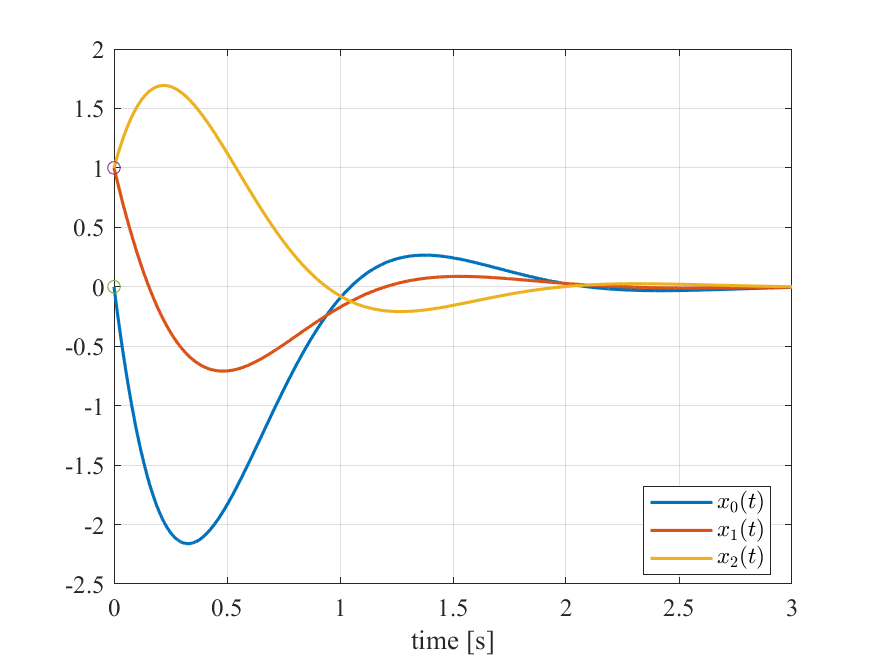
\includegraphics[width=1.0\textwidth]{observability2.png}
  \caption{Состояния системы}
\end{figure}

Как можно заметить, они совпадают с моделированием вектора состояний.
\newpage
Теперь проведём моделирование с начальными условиями x(0), без управления: на рисунке ниже видно,
что выход системы совпадает с функцией y(t) выше заданной. Ошибка наблюдения достаточно мала и не превышает $10^{-10}$.

\begin{figure}[ht]
    \centering
    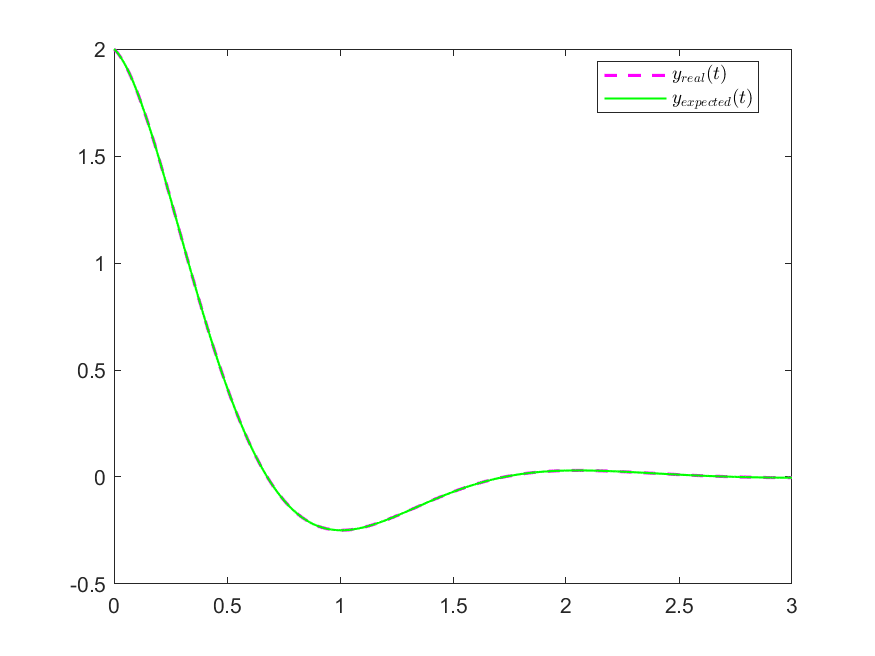
\includegraphics[width=1.0\textwidth]{output2.png}
    \caption{Выход системы}
  \end{figure}

\begin{figure}[ht]
    \centering
    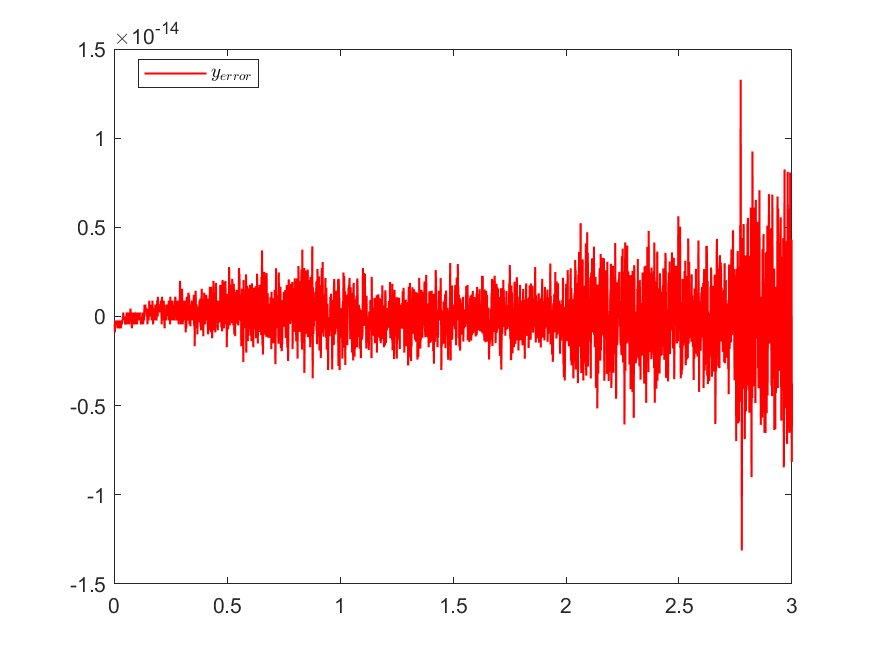
\includegraphics[width=1.0\textwidth]{error2.png}
    \caption{Ошибка выхода системы}
  \end{figure}

\newpage
\newpage
\subsection{Альтернативные начальные условия}

Так как система не является полностью наблюдаемой, то мы можем найти бесконечное количество начальных условий,
при которых выход системой будет совпадать с исходной $y(t) = f(t)$. Чтобы найти это множество, нам нужно найти \text{nullspace} ядра матрицы наблюдаемости $V$:
$$
\text{Nullspace}(V) = \begin{Bmatrix}
    \begin{bmatrix}
        -0.57\\-0.57\\0.57
    \end{bmatrix}
\end{Bmatrix} 
$$
Тогда общее множества "ненаблюдаемых" начальных условий можно выразить как линейную комбинацию:
$$
    x^*(0) = x(0) + \beta \begin{bmatrix}
                            -0.57\\-0.57\\0.57
                            \end{bmatrix}
$$
Выберем следующие значения коэффициента:
$$
    \begin{aligned}
        \beta_1=1, \tab x^*_1(0) = \begin{bmatrix}
            -0.57\\0.42\\1.57
        \end{bmatrix} \\
        \beta_2=5, \tab x^*_2(0) = \begin{bmatrix}
            -2.88\\-1.88\\3.88
        \end{bmatrix} \\
        \beta_3=100, \tab x^*_3(0) = \begin{bmatrix}
            -57.73\\-56.73\\58.73
        \end{bmatrix}
    \end{aligned}
$$
Теперь проведём моделирование с этими начальными условиями и убедимся в том, что выход у всех этих систем будет идентичный\dots
\newpage
\begin{figure}[ht]
\centering
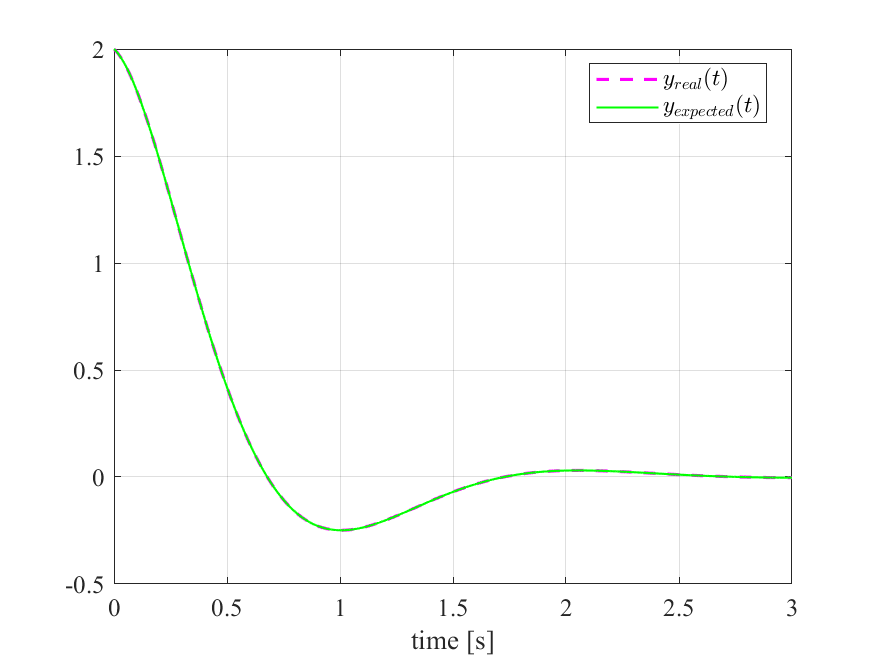
\includegraphics[width=0.8\textwidth]{output3.png}
\caption{Выход системы с начальными условиями $x^*_1(0)$}
\end{figure}
\begin{figure}[ht]
\centering
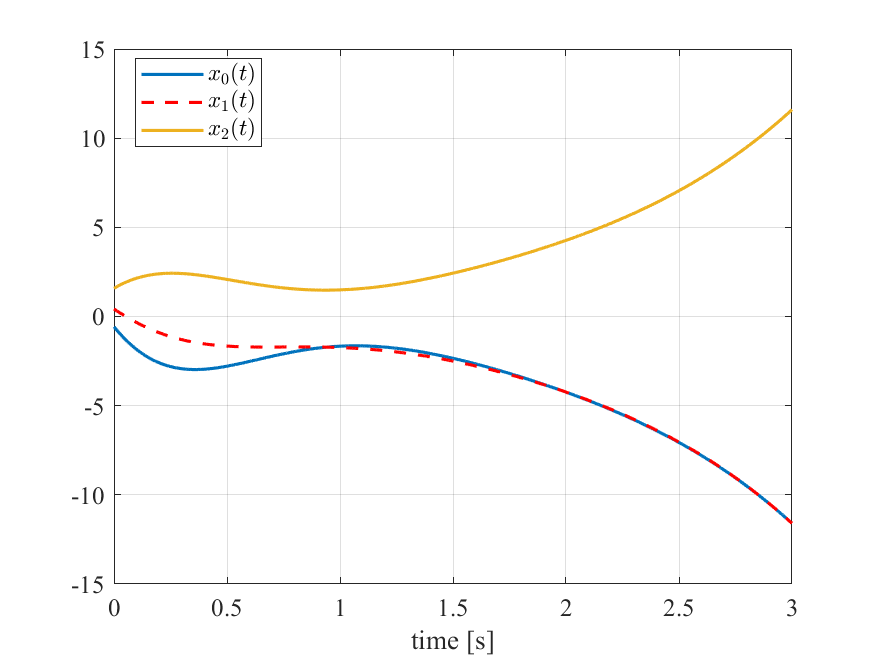
\includegraphics[width=0.8\textwidth]{observability3.png}
\caption{Состояние системы с начальными условиями $x^*_1(0)$}
\end{figure}
\newpage
\begin{figure}[ht]
\centering
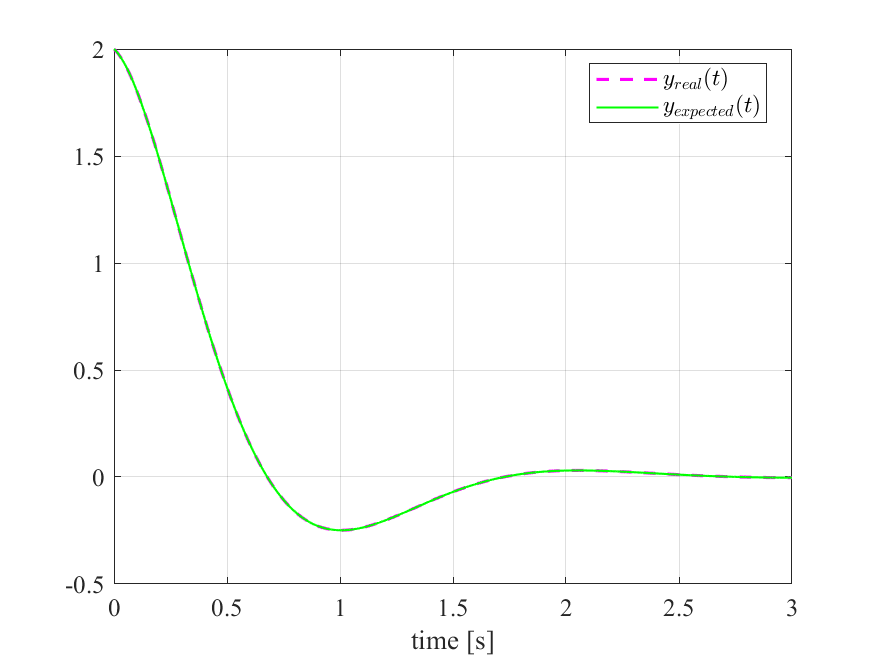
\includegraphics[width=0.8\textwidth]{output4.png}
\caption{Выход системы с начальными условиями $x^*_2(0)$}
\end{figure}
\begin{figure}[ht]
\centering
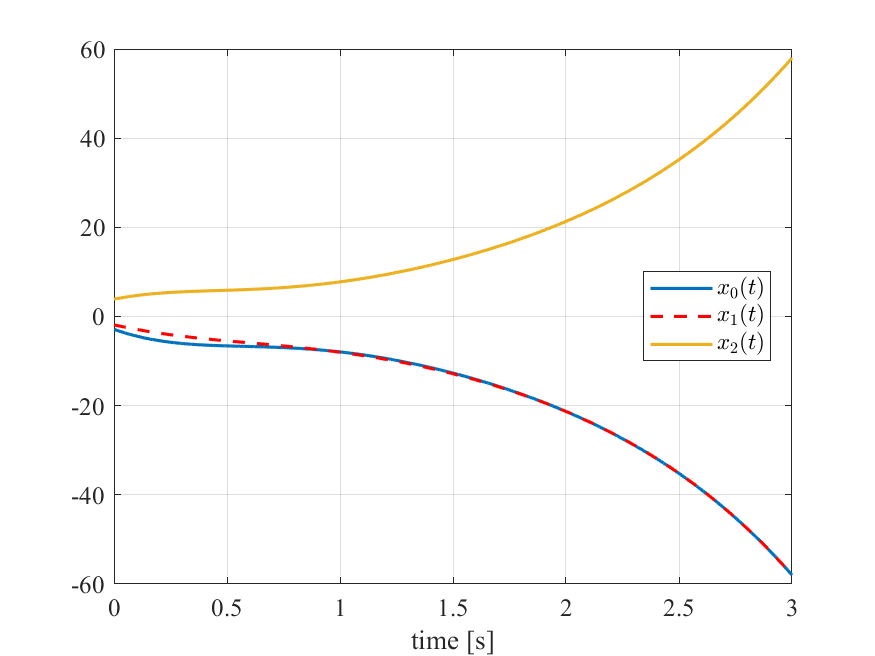
\includegraphics[width=0.8\textwidth]{observability4.png}
\caption{Состояние системы с начальными условиями $x^*_2(0)$}
\end{figure}

\newpage
\begin{figure}[ht]
\centering
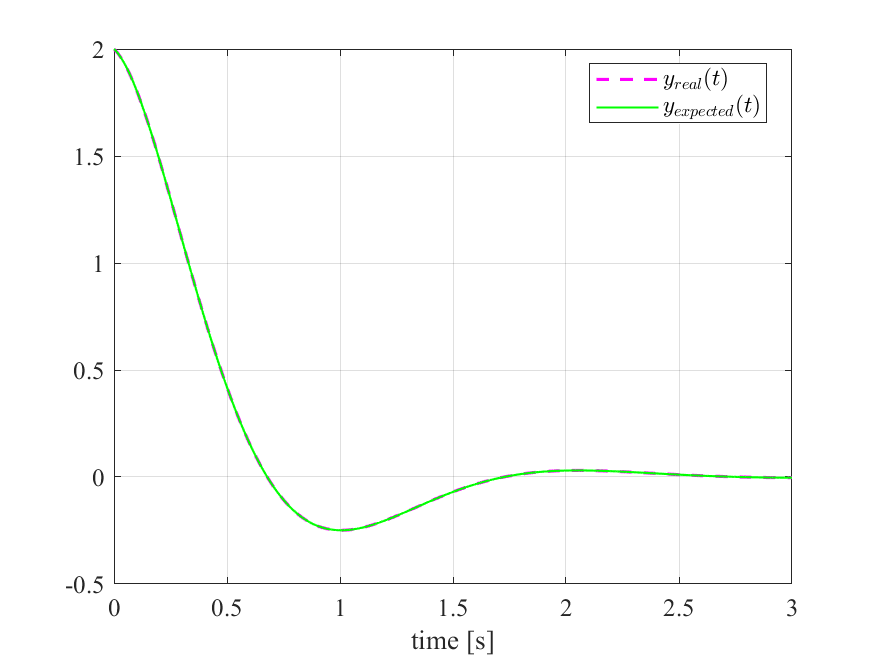
\includegraphics[width=0.8\textwidth]{output5.png}
\caption{Выход системы с начальными условиями $x^*_3(0)$}
\end{figure}
\begin{figure}[ht]
\centering
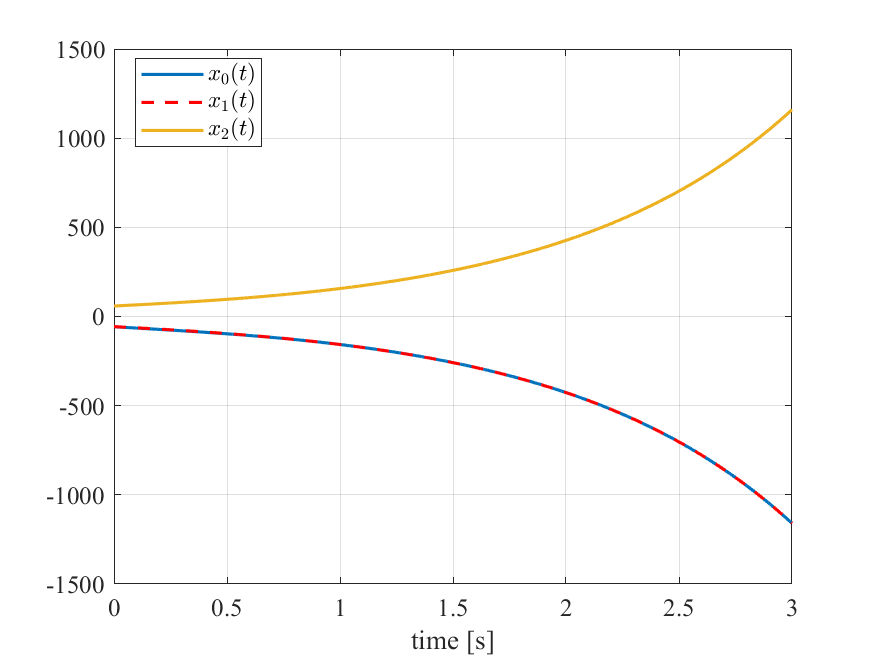
\includegraphics[width=0.8\textwidth]{observability5.png}
\caption{Состояние системы с начальными условиями $x^*_3(0)$}
\end{figure}



\newpage
\subsection{Вывод}

В этом задании мы исследовали не полностью наблюдаемую систему, это мы увидели
с помощью матрицы  наблюдаемости, критерия Калмана, через наблюдаемость собственных значений и жорданову форму системы.
Также был найден грамиан наблюдаемости и проверены его собственные числа. 
Провели моделирование системы с начальными условиями, при которых выход системы совпадает
с заданной функцией. Нам удалось показать, что для не полностью наблюдаемых систем есть пространство "ненаблюдаемых" начальных условий, при которых
выходы систем не будут отличаться друг от друга, и по траектории $y(t)$ в таком случае мы не сможем однозначно восстановить $x(0)$.

\endinput